\chapter[Implementering af mekanik]{Mekanik}
\mnote{Nick Østergaard}

% Note om hvad der skal stå i dette afsnit her.
% Kort afsnit om hvordan vi har lavet vores produkt ud fra vores
% overvejelser

Figur \fixme{Indsæt figur over færdigt produkt} viser vores færdige
produkt.  Udformningen af produktet tager udgangspunkt i vores
overvejelser i design-afsnittet.  Man ser ud fra figuren, at akserne
styres af to stepmotor, som er henholdsvis uni- og bipolar.  Vi
startede med at lave basen for vores produkt. Her tog vi udgangspunkt
i, at vi skulle kunne tegne på et stykke A4-papir. Yderligere havde vi
brug for plads til vores hardware, som styrer stepmotorerne. Herefter
blev gliderne og deres respektive dele lavet og sat sammen med basen,
som det fremgår af figuren. Vi havde brug for en holder til pennen,
som passede med gliderne, så det var naturligt at lave denne i den
afsluttende del af produktionsforløbet.

\section{Tegnehovedet}\fixme{Under mekansik}
Tegnehoved er i afsnittet\vref{sc:d-tegnehoved} beskrevet som en
penholder. Vores tegnehoved er konstrueret som det ses på
figur\vref{fig:tegnehoved-skitse}.

På en glider, er der monteret en trækmagnet, som er forbundet mekanisk
til en arm der holder pennen. Armen holdes oppe af en fjeder. Når man
aktiverer trækmagneten, vil

\begin{figure}[htbp]
  \centering
  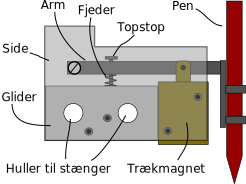
\includegraphics[width=7cm]{./img/tegnehoved-skitse}
  \caption{Skitse af tegnehoved}
  \label{fig:tegnehoved-skitse}
\end{figure}

\mnote{
  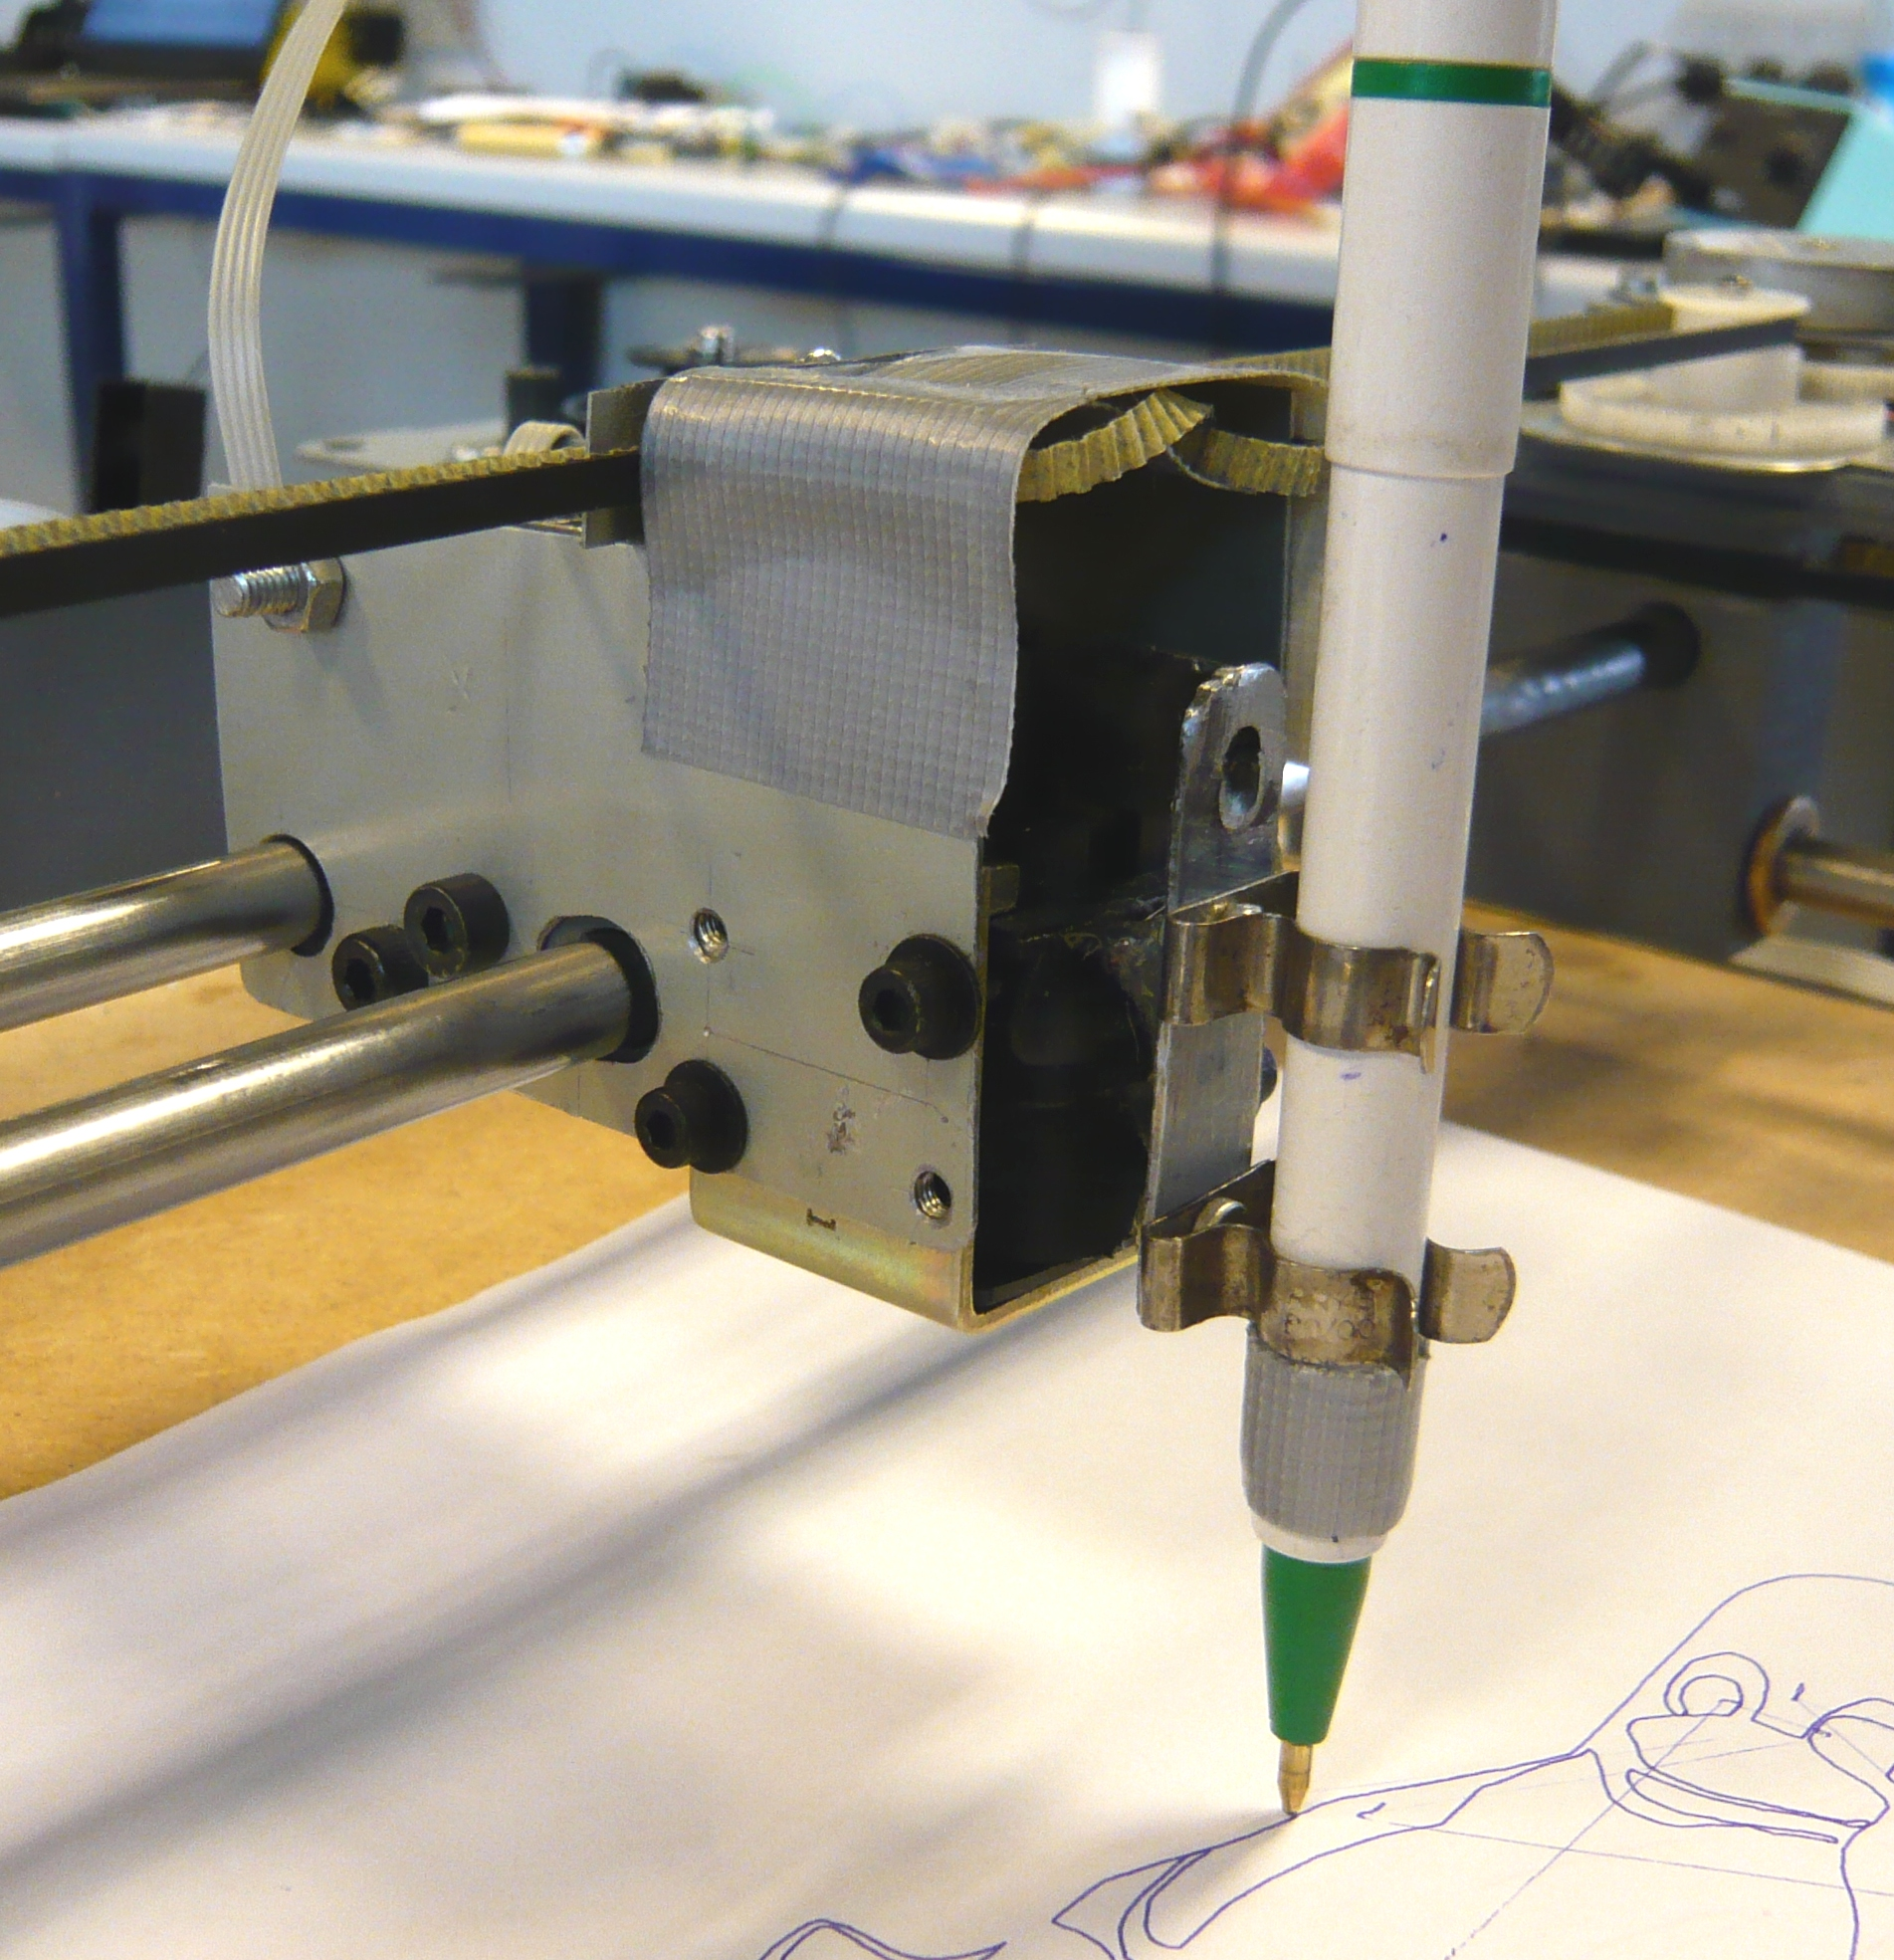
\includegraphics[width=\marginparwidth]{./img/tegnehoved}
  \captionof{figure}{Tegne\-hovedet i dets reele form}
  \label{fig:tegnehoved}
}

%%% Local Variables: 
%%% mode: latex
%%% TeX-master: "../master"
%%% End: 